  \documentclass{beamer}

% Used packages
\usepackage[utf8]{inputenc}
\usepackage[spanish]{babel}
\usepackage{amssymb, amsmath, amsthm, amsfonts, esint, mathtools}




% There are many different themes available for Beamer. A comprehensive
% list with examples is given here:
% http://deic.uab.es/~iblanes/beamer_gallery/index_by_theme.html
% You can uncomment the themes below if you would like to use a different
% one:
%\usetheme{AnnArbor}
\usetheme{Antibes}
%\usetheme{Bergen}
%\usetheme{Berkeley}
%\usetheme{Berlin}
%\usetheme{Boadilla}
%\usetheme{boxes}
%\usetheme{CambridgeUS}
%\usetheme{Copenhagen}
%\usetheme{Darmstadt}
%\usetheme{default}
%\usetheme{Frankfurt}
%\usetheme{Goettingen}
%\usetheme{Hannover}
%\usetheme{Ilmenau}
%\usetheme{JuanLesPins}
%\usetheme{Luebeck}
%\usetheme{Madrid}
%\usetheme{Malmoe}
%\usetheme{Marburg}
%\usetheme{Montpellier}
%\usetheme{PaloAlto}
%\usetheme{Pittsburgh}
%\usetheme{Rochester}
%\usetheme{Singapore}
%\usetheme{Szeged}
%\usetheme{Warsaw}

\title{Clump Detection and Organization through MRA}

% A subtitle is optional and this may be deleted
\subtitle{A 3D Discrete Wavelet Transform Application}

\author{Martín Villanueva\inst{1}}
% - Give the names in the same order as the appear in the paper.
% - Use the \inst{?} command only if the authors have different
%   affiliation.

\institute[Universidad Técnica Federico Santa María] % (optional, but mostly needed)
{
  \inst{1}%
  Departamento de Informática\\
  Universidad Técnica Federico Santa María}
% - Use the \inst command only if there are several affiliations.
% - Keep it simple, no one is interested in your street address.

\date{Astroinformática, 2016}
% - Either use conference name or its abbreviation.
% - Not really informative to the audience, more for people (including
%   yourself) who are reading the slides online

%\subject{Theoretical Computer Science}
% This is only inserted into the PDF information catalog. Can be left
% out.

% If you have a file called "university-logo-filename.xxx", where xxx
% is a graphic format that can be processed by latex or pdflatex,
% resp., then you can add a logo as follows:

% \pgfdeclareimage[height=0.5cm]{university-logo}{university-logo-filename}
% \logo{\pgfuseimage{university-logo}}

% Delete this, if you do not want the table of contents to pop up at
% the beginning of each subsection:
\AtBeginSubsection[]
{
  \begin{frame}<beamer>{Outline}
    \tableofcontents[currentsection,currentsubsection]
  \end{frame}
}

% Let's get started
\begin{document}

\begin{frame}
  \titlepage
\end{frame}



\begin{frame}{Outline}
  \tableofcontents
  % You might wish to add the option [pausesections]
\end{frame}




% Section and subsections will appear in the presentation overview
% and table of contents.
\section{Introducción}

\subsection{Wavelets}

\begin{frame}{What is a Wavelet? (2)}
Wavelets are just mathematical functions $\Psi(t)$ with interesting properties:

\begin{itemize}
    \item  They have a band-pass like spectrum: $|\boldsymbol{\Psi}(\boldsymbol{\omega})|^2 \bigg|_{\boldsymbol{\omega}=0} = 0$
    \item $\int \Psi(t) dt = 0 \rightarrow$ mean value of zero and therefore must be oscillatory (\textit{A wave!}).
    \item They have concentration in both time and frequency domains (\textit{Compact Support!})
    \item The last one is achieved through the \textit{Vanishing Moments} condition: $\int t^p \phi(t) dt = 0$
\end{itemize}
\end{frame}

\begin{frame}{What is a Wavelet? (3)}
\begin{figure}[htpb!]
\centering
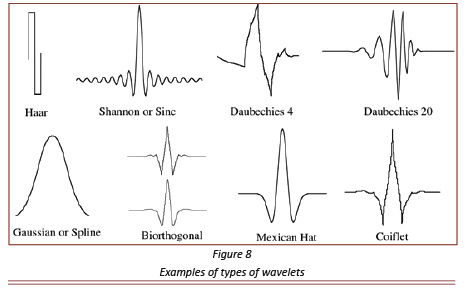
\includegraphics[width=10cm]{wav_ex}
\end{figure}    
\end{frame}

\begin{frame}{Continuous Wavelet Transform}
\textbf{Idea:} Decomposing a signal function $f(t)$ into a set of basis wavelet functions $\Psi_{s,\tau}(t)$:
$$ \gamma(s, \tau) = \int f(t) \Psi_{s, \tau}(t)^{*} dt $$
where $s$ and $\tau$ are the scale and translation. We can then reconstruct the original signal by the inverse process:
$$ f(t) = \int \int \gamma(s,\tau) \Psi_{s,\tau}(t) d\tau d s$$
Here the wavelets are dilated and expanded versions of the so-called \textbf{mother wavelet} $\Psi(t)$:
$$ \Psi_{s, \tau}(t) = \frac{1}{\sqrt{s}} \Psi \left(\frac{t-\tau}{s} \right)$$
\end{frame}


\begin{frame}{Discrete Wavelet Transform}
Most of times, CWT can't be obtained analytically. So we have to discretize and compute it numerically. Discrete Wavelets can only be scaled and translated in discrete steps:
$$\Psi_{j,k}(t) = \frac{1}{\sqrt{s_0^j}} \Psi \left(\frac{t - k \tau_0 s_0^j}{s_0^j} \right)$$
and then an arbitrary signal can be reconstructed by:
$$ f(t) = \sum_{j,k} \gamma(j,k) \Psi_{j,k}(t) $$

\textbf{Problem}: It still needs an infinite number of wavelets!
\end{frame}


\begin{frame}{Discrete Wavelet Transform (2)}
\textbf{Solution:} The scaling function!

\begin{figure}[htpb!]
\centering
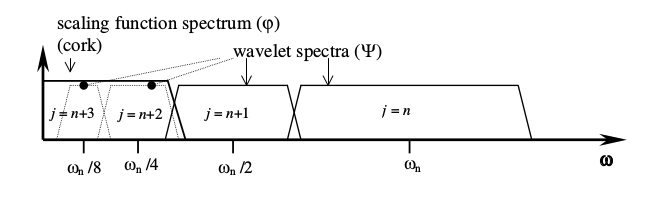
\includegraphics[width=10cm]{scaling_function}
\caption{Filter Bank Decomposition}
\end{figure}

\begin{itemize}
    \item Each wavelet has a band-pass spectrum.
    \item We will not cover the spectrum all way down to zero, but to use a low-pass filter to plug the hole
    when it is small enough.
\end{itemize}
        
\end{frame}


\subsection{Multi-Resolution Analysis (MRA)}
\begin{frame}{Subband Coding}
\textbf{Idea:} We can see the DWT as a filter bank, that passes the signal through
this filter bank, and the output of the different filter stages are the wavelet -and
scaling function- coefficients.
\begin{figure}[htpb!]
\centering
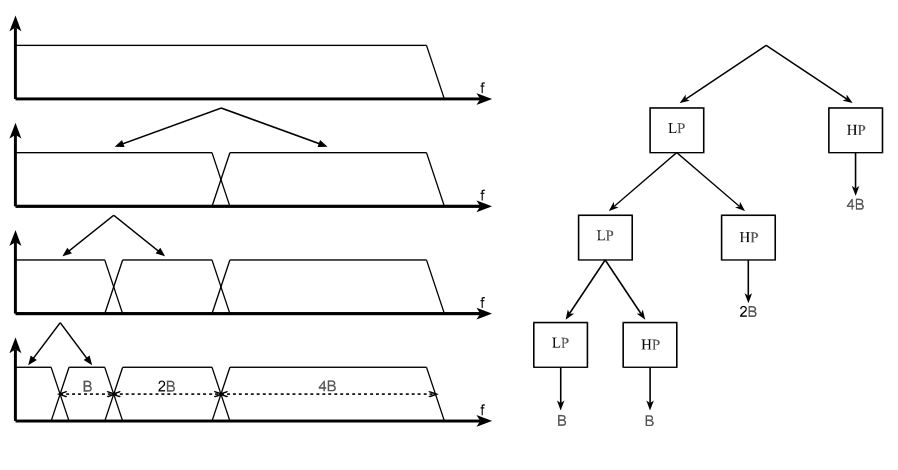
\includegraphics[width=9cm]{mra}
\caption{Subband Coding}
\end{figure}

    
\end{frame}


\subsection{State of the Art}

\begin{frame}{Alves et al.}

\begin{figure}[htpb!]
\centering

\includegraphics[width=9cm]{alves}
\end{figure}

\textbf{Procedure:} \textit{Object identification in wavelet space}:
For a given scale $i$, structures are isolated with \textbf{classical thresholding}
at $i$ with $\sigma_i$ being the noise amplitude at scale $i$. A structure at scale
$i$ is connected with a structure at scale $i+1$ if its local maxima drops in structure
at scale $i +1$.

\textbf{Observation:} It uses a different approach of DWT, called the Stationary Wavelet Transform
(SWT). Given some image, it produces a \textit{redundant} representation on the Wavelet space, and
of the \textit{same size} of the input image.
\end{frame}



\begin{frame}{Gregorio et al.}

\begin{figure}[htpb!]
\centering
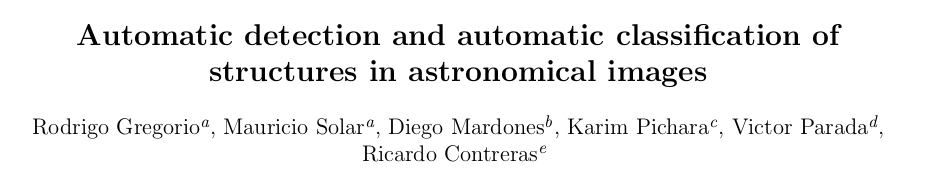
\includegraphics[width=9cm]{gregorio}
\end{figure}

\textbf{Procedure:} Similar to Alves, computes SWT of 2D image at different scales, but
finding structures in the Wavelet space through a clump identification algorithm (like
ClumpFind).

\begin{figure}[htpb!]
\centering
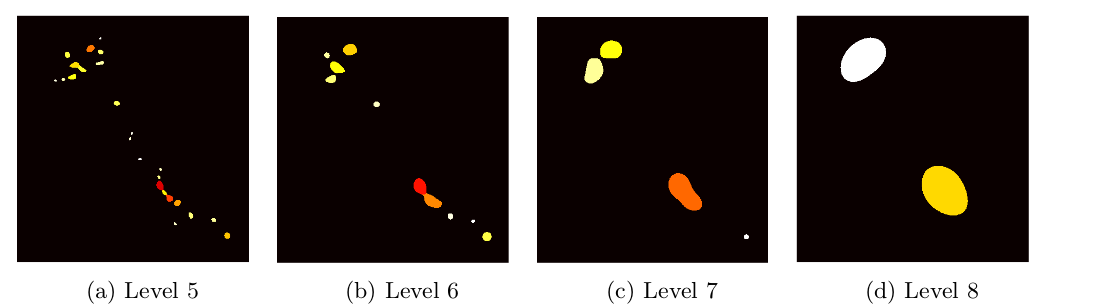
\includegraphics[width=10cm]{gregorio_mra}
\end{figure}

\end{frame}



\section{Proposal}

\subsection{Proposed Project}

\begin{frame}{Project}

\textbf{Motivation:} Precisely represent the dense core formations in cold molecular clouds,
and its structural relationship.

\begin{itemize}
  \item Extend the ideas of Gregorio to 3D, so we can work with 3D Spectroscopic
  Data Cubes directly.
  \item This will be achieved by MRA with 3D Discrete Wavelet Transform.
  \item The isolation Steps will be carried out by algorithms like ClumpFind or FellWalker.
  \item The results on different levels will be summarized in a Dendrogram tree structure.
\end{itemize}
\end{frame}


\begin{frame}{Project: Limitations}
\begin{itemize}
  \item Using 3D SWT would be terrible inefficient! As we have seen, it produces a redundant
  representation of the \textit{same size} of the input. (\textit{An sparse representation
  is needed!})
  \item SWT for 3D wavelets isn't implemented in any software package anyway.
  \item We have to choose the 3D wavelet(s) (or build one) that bests extract/represents
  the needed features.  
\end{itemize}
\end{frame}

\begin{frame}{Project: Solution}
We can use a DWT (with no redundance), which can be seen as a sparse representation
of an image. Then there are two options:
\begin{itemize}
  \item At each level, Find out a way to find structures on the Wavelet space.
  \item At each level, compute the IDWT and find structure on this resampled version
  of the image.
\end{itemize}
\end{frame}


\subsection{Technical Details}
\begin{frame}{Technical Details}
Solution will be implemented in Matlab. Why?
\begin{itemize}
  \item It has the best and more serious Wavelet software package.
  \item And it has (almost )all the other necessary stuff: Fits routines,
  Dendrograms software, etc.
  \item But, it will be necessary to implement or integrate clump detection
  algorithms.
\end{itemize} 
\end{frame}






\end{document}